% !TeX program = xelatex
\documentclass[a4paper,10pt]{article}

% ============================================================================
% សន្លឹកកិច្ចការសិស្សបំពេញចន្លោះ ស-ខ្មៅ និងប្លង់ក្ដារខៀន/ចម្លើយគ្រូ (គ្មាន LCD / គ្មានកន្ត្រៃ)
% មេរៀនទី៦ (៤)៖ វិធីគុណនិងវិធីចែកកន្សោមសនិទាន — ត្រូវគ្នានឹង LS_Plan_RAT63.tex
% ============================================================================
\usepackage[a4paper, left=1.0cm, right=1.0cm, top=0.75cm, bottom=1.00cm, footskip=0.52cm]{geometry}
\usepackage{amsmath}
\usepackage{unicode-math}
\usepackage{fontspec}
\usepackage{array, colortbl}
\usepackage[table]{xcolor}
\usepackage{enumitem}
\usepackage{pifont}
\usepackage{fancyhdr}
\usepackage{lastpage}
\usepackage{tikz}
\usepackage[most]{tcolorbox}
\usetikzlibrary{calc, arrows.meta, decorations.pathreplacing, positioning, babel}

\makeatletter
\let\@expl@@@mark@update@singlecol@structures@@\relax
\makeatother

\providecommand{\NGSFindFonts}{%
  \IfFileExists{C:/Windows/Fonts/cambria.ttc}{%
    \def\NGSSysPath{C:/Windows/Fonts/}%
    \def\NGSUserPath{C:/Users/KIT/AppData/Local/Microsoft/Windows/Fonts/}%
  }{%
    \IfFileExists{./fonts/KhmerOSsiemreap.ttf}{\def\NGSSysPath{./fonts/}\def\NGSUserPath{./fonts/}}{%
    \IfFileExists{../fonts/KhmerOSsiemreap.ttf}{\def\NGSSysPath{../fonts/}\def\NGSUserPath{../fonts/}}{%
    \IfFileExists{../../fonts/KhmerOSsiemreap.ttf}{\def\NGSSysPath{../../fonts/}\def\NGSUserPath{../../fonts/}}{%
    \IfFileExists{../../../fonts/KhmerOSsiemreap.ttf}{\def\NGSSysPath{../../../fonts/}\def\NGSUserPath{../../../fonts/}}{%
    \IfFileExists{../../../../fonts/KhmerOSsiemreap.ttf}{\def\NGSSysPath{../../../../fonts/}\def\NGSUserPath{../../../../fonts/}}{%
    \IfFileExists{../../../../../fonts/KhmerOSsiemreap.ttf}{\def\NGSSysPath{../../../../../fonts/}\def\NGSUserPath{../../../../../fonts/}}{%
    \IfFileExists{../../../../../../fonts/KhmerOSsiemreap.ttf}{\def\NGSSysPath{../../../../../../fonts/}\def\NGSUserPath{../../../../../../fonts/}}{%
      \def\NGSSysPath{../../../../../../../fonts/}\def\NGSUserPath{../../../../../../../fonts/}%
    }}}}}}}%
  }%
}
\NGSFindFonts

\setmathfont[Path={\NGSSysPath}, FontIndex=1, Scale=1.02]{cambria.ttc}
\defaultfontfeatures{Ligatures=TeX}

\setmainfont[
  Path={\NGSUserPath}, Extension=.ttf, Script=Khmer,
  BoldFont={KhmerOSsiemreap}, BoldFeatures={FakeBold=1.8},
  ItalicFont={KhmerOSsiemreap}, ItalicFeatures={FakeSlant=0.25},
  BoldItalicFont={KhmerOSsiemreap}, BoldItalicFeatures={FakeBold=1.8, FakeSlant=0.25}
]{KhmerOSsiemreap}

\newfontfamily\muol[Path={\NGSUserPath}, Extension=.ttf, Script=Khmer]{KhmerOSmuollight}
\newfontfamily\TimesEn[Path={\NGSSysPath}, Extension=.ttf, BoldFont={timesbd}, ItalicFont={timesi}, BoldItalicFont={timesbi}]{times}
\newfontfamily\CalibriFont[Path={\NGSSysPath}, Extension=.ttf]{calibri}

\XeTeXlinebreaklocale "km"
\XeTeXlinebreakskip = 0pt plus 1pt minus 0.1pt

\definecolor{panelgray}{gray}{0.94}
\definecolor{headgray}{gray}{0.85}

\pagestyle{fancy}
\fancyhf{}
\renewcommand{\headrulewidth}{0pt}
\fancyfoot[L]{\fontsize{7.4pt}{9.5pt}\selectfont អនុវិទ្យាល័យព្រះក្រសាំង \en{|} គ្រូ៖ ហុក ប៊ុនថែន \en{|} មេរៀនទី៦ (៤) វិធីគុណនិងវិធីចែកកន្សោមសនិទាន \en{|} ថ្ងៃពុធ ទី១៦ ខែធ្នូ ឆ្នាំ២០២៦}
\fancyfoot[R]{\fontsize{7.8pt}{10pt}\selectfont ទំព័រ \en{\thepage\ / \pageref{LastPage}}}

\setlength{\parindent}{0pt}
\setlength{\parskip}{0pt}
\setlength{\tabcolsep}{4pt}

\newcommand{\en}[1]{{\TimesEn #1}}
\newcommand{\enbf}[1]{{\TimesEn\bfseries #1}}
\newcommand{\unit}[1]{\,\text{\en{#1}}}
\newcommand{\riel}{\,\text{៛}}
\newcommand{\cnum}[1]{\mbox{\fontsize{10pt}{12pt}\selectfont\ding{\numexpr181+#1\relax}}}
\newcommand{\chkbox}{\tikz[baseline=-0.15ex]\draw[black, line width=0.85pt, fill=white] (0,0) rectangle (0.24cm,0.24cm);}
\newcommand{\ansbox}[1][2.0cm]{\,\tikz[baseline=-0.65ex]\draw[black, line width=0.65pt, fill=white] (0,0) rectangle (#1, 0.42cm);\,}
\newcommand{\dotline}[1][2.2cm]{\makebox[#1]{\dotfill}}

\newcommand{\pagebanner}[2]{%
  \begin{tcolorbox}[
    enhanced, sharp corners, colback=headgray, colframe=black,
    boxrule=1.05pt, boxsep=1pt, top=2.5pt, bottom=2.5pt, left=6pt, right=6pt,
    after skip=3.5pt
  ]
    {\muol\fontsize{9.0pt}{13.2pt}\selectfont #1}\hfill{\fontsize{8.0pt}{11.2pt}\selectfont\textbf{#2}}
  \end{tcolorbox}%
}

\newcommand{\secstrip}[2]{%
  \vspace{3pt}%
  \begin{tcolorbox}[
    enhanced, sharp corners, colback=panelgray, colframe=black,
    boxrule=0.8pt, boxsep=0.8pt, top=2pt, bottom=2pt, left=5pt, right=5pt,
    after skip=3pt
  ]
    {\muol\fontsize{8.5pt}{12.2pt}\selectfont #1}\hfill{\fontsize{7.8pt}{10.8pt}\selectfont\textit{#2}}
  \end{tcolorbox}%
}

\newcolumntype{L}[1]{>{\raggedright\arraybackslash}p{#1}}
\newcolumntype{C}[1]{>{\centering\arraybackslash}p{#1}}

\begin{document}
\fontsize{9.5pt}{14.5pt}\selectfont

% ============================================================================
% ទំព័រទី ១៖ សន្លឹកកិច្ចការសិស្ស (ផ្នែកមុខ៖ E1 -> E2 -> E3)
% ============================================================================
\pagebanner{សន្លឹកកិច្ចការសិស្ស \enbf{(}៦\enbf{.}៤ វិធីគុណនិងវិធីចែកកន្សោមសនិទាន\enbf{)} \enbf{--} ផ្នែកមុខ}{ថ្នាក់ទី៨ \en{|} ទំ.៧៨--៨០}

\begin{tcolorbox}[
  enhanced, sharp corners, colback=white, colframe=black,
  boxrule=0.8pt, boxsep=1.5pt, top=3.5pt, bottom=3.5pt, left=5pt, right=5pt,
  after skip=4pt
]
  \fontsize{9.0pt}{13.0pt}\selectfont
  \textbf{ឈ្មោះសិស្ស៖} \dotline[4.3cm] \quad
  \textbf{សមាជិកក្រុម៖} \dotline[4.3cm] \quad
  \textbf{ថ្នាក់ទី៖} ៨\dotline[0.9cm] \quad
  \textbf{ក្រុមទី៖} \dotline[1.0cm]
\end{tcolorbox}

% --- E1 Engage ---
\secstrip{ផ្នែកទី ១ \enbf{(E1 - Engage)} ៖ បេសកកម្មចាប់កំហុសសម្រួលមុនប្ដូរសញ្ញាចែក}{រយៈពេល ៣ នាទី (គូស \ding{51} ក្នុង \chkbox)}

\begin{tcolorbox}[
  enhanced, sharp corners, colback=white, colframe=black,
  boxrule=0.8pt, boxsep=2.5pt, top=4pt, bottom=4pt, left=6pt, right=6pt
]
  គេចង់គណនាផលចែក $\dfrac{a^2 - 9}{3a} \div \dfrac{a + 3}{a - 3}$ (ទំ.៨០) ។ តើសិស្សរូបណាគណនាបានត្រឹមត្រូវ?\\[3pt]
  \chkbox\ \textbf{សិស្ស ក៖} ឈូត $(a-3)$ និង $(a+3)$ ភ្លាម បាន $\dfrac{1}{3a}$ \qquad
  \chkbox\ \textbf{សិស្ស ខ៖} គុណនឹងចម្រាសតួចែក បាន $\dfrac{(a - 3)^2}{3a}$\\[3pt]
  $\bullet$ \textbf{តេស្តដោយជំនួស $a = 6$៖} កន្សោមដើមស្មើ $\dfrac{27}{18} \div \dfrac{9}{3} = \dfrac{1}{2}$; \ ចម្លើយសិស្ស ក ស្មើ \ansbox[1.7cm]; \ សិស្ស ខ ស្មើ \ansbox[1.7cm] ។
\end{tcolorbox}

\vspace{3pt}

% --- E2 Explore ---
\secstrip{ផ្នែកទី ២ \enbf{(E2 - Explore)} ៖ វិធីគុណ និងវិធីចែកកន្សោមសនិទាន (ទំ.៧៨--៨០)}{រយៈពេល ១១ នាទី}

\textbf{សកម្មភាព ១ (\en{E2-A} — ៥ នាទី)៖ ៤.១ វិធីគុណកន្សោមសនិទាន (ទំ.៧៨--៧៩ ឧទាហរណ៍ទី ១ និងទី ២)}

\begin{tcolorbox}[
  enhanced, sharp corners, colback=white, colframe=black,
  boxrule=0.8pt, boxsep=2.5pt, top=4pt, bottom=4pt, left=6pt, right=6pt
]
  $\bullet$ \textbf{១) ឧទាហរណ៍ទី ១៖} $\dfrac{7b}{10a} \times \dfrac{5a^2}{8b} = \dfrac{35a^2b}{80ab} \longrightarrow$ សម្រួលនឹង $5ab$ បាន \ansbox[2.6cm]\\[4pt]
  $\bullet$ \textbf{២) ឧទាហរណ៍ទី ២៖} $\dfrac{5x}{4x - 12} \times \dfrac{2x^2 - 6x}{3} = \dfrac{5x}{4(x - 3)} \times \dfrac{2x(x - 3)}{3} =$ \ansbox[2.8cm]
\end{tcolorbox}

\vspace{4pt}
\textbf{សកម្មភាព ២ (\en{E2-B} — ៦ នាទី)៖ ៤.២ វិធីចែកកន្សោមសនិទាន (ទំ.៧៩--៨០ ឧទាហរណ៍ ក និង ខ)}

\begin{tcolorbox}[
  enhanced, sharp corners, colback=white, colframe=black,
  boxrule=0.8pt, boxsep=2.5pt, top=4pt, bottom=4pt, left=6pt, right=6pt
]
  $\bullet$ \textbf{១) ឧទាហរណ៍ ក៖} $\dfrac{4x^2}{15y} \div \dfrac{3x}{10y^2} = \dfrac{4x^2}{15y} \times \dfrac{10y^2}{3x} = \dfrac{40x^2y^2}{45xy} =$ \ansbox[2.8cm]\\[4pt]
  $\bullet$ \textbf{២) ឧទាហរណ៍ ខ៖} $\dfrac{a^2 - 9}{3a} \div \dfrac{a + 3}{a - 3} = \dfrac{(a - 3)(a + 3)}{3a} \times \dfrac{a - 3}{a + 3} =$ \ansbox[3.0cm]
\end{tcolorbox}

\vfill

% --- E3 Explain ---
\secstrip{ផ្នែកទី ៣ \enbf{(E3 - Explain)} ៖ សង្ខេបវិធានគុណ-ចែក និងធនាគារហេតុផល \enbf{B\&W}}{រយៈពេល ៦ នាទី}

\begin{tcolorbox}[
  enhanced, sharp corners, colback=white, colframe=black,
  boxrule=0.85pt, boxsep=2.5pt, top=4pt, bottom=4pt, left=6pt, right=6pt
]
  $\bullet$ \textbf{១) វិធានវិធីគុណ៖} ដាក់ជាផលគុណកត្តាសិន រួចគុណភាគយកនឹងភាគយក ភាគបែងនឹងភាគបែង៖ $\dfrac{A}{B} \times \dfrac{C}{D} =$ \ansbox[2.0cm]\\[4pt]
  $\bullet$ \textbf{២) វិធានវិធីចែក៖} គុណប្រភាគតំណាងចែកនឹងចម្រាសនៃប្រភាគតួចែក៖ $\dfrac{A}{B} \div \dfrac{C}{D} = \dfrac{A}{B} \times$ \ansbox[1.8cm] $=$ \ansbox[2.0cm]\\[4pt]
  \tikz\draw[black, dashed, line width=0.6pt] (0,0) -- (\linewidth,0);\\[3pt]
  \fontsize{8.8pt}{13.0pt}\selectfont
  \textbf{ធនាគារហេតុផល (\en{Warrant Bank})៖} \quad
  \cnum{1} ដាក់ជាផលគុណកត្តាសិនមុនគុណពង្រីក\\
  \cnum{2} ត្រឡប់តែប្រភាគតួចែក ($\tfrac{C}{D} \to \tfrac{D}{C}$) \quad
  \cnum{3} ហាមសម្រួលឆ្លងសញ្ញា $(\div)$ \quad
  \cnum{4} ពហុធា $P = \tfrac{P}{1}$ មានចម្រាស $\tfrac{1}{P}$
\end{tcolorbox}

% ============================================================================
% ទំព័រទី ២៖ សន្លឹកកិច្ចការសិស្ស (ផ្នែកខាងខ្នង៖ E4 -> E5 -> កិច្ចការផ្ទះ)
% ============================================================================
\clearpage
\pagebanner{សន្លឹកកិច្ចការសិស្ស \enbf{(}៦\enbf{.}៤ វិធីគុណនិងវិធីចែកកន្សោមសនិទាន\enbf{)} \enbf{--} ផ្នែកខ្នង}{ថ្នាក់ទី៨ \en{|} ទំ.៧៩--៨០, ៨៦}

% --- E4 Elaborate ---
\secstrip{ផ្នែកទី ៤ \enbf{(E4 - Elaborate)} ៖ លំហាត់គំរូវិធីគុណ និងវិធីចែក (ទំ.៧៩--៨០)}{រយៈពេល ១០ នាទី}

\begin{tcolorbox}[
  enhanced, sharp corners, colback=white, colframe=black,
  boxrule=0.8pt, boxsep=2.5pt, top=4pt, bottom=4pt, left=6pt, right=6pt
]
  \textbf{១) លំហាត់គំរូវិធីគុណ (ទំ.៧៩)៖}\\[3pt]
  \hspace*{0.3cm}$\bullet$ ក៖ $\dfrac{a^2 - 2a + 1}{a^2 - 1} \times \dfrac{a^2 + a}{a^2 - 2a} =$ \ansbox[2.8cm] \quad
  ខ៖ $\dfrac{m^2 + 6m + 9}{(a + 2b)^2} \times \dfrac{7a + 14b}{m + 3} =$ \ansbox[3.0cm]\\[4pt]
  \textbf{២) លំហាត់គំរូវិធីចែក (ទំ.៨០)៖}\\[3pt]
  \hspace*{0.3cm}$\bullet$ ក៖ $\dfrac{a + 3}{b^2 + 4b + 4} \div \dfrac{2a + 6}{b + 2} =$ \ansbox[2.8cm] \quad
  ខ៖ $\dfrac{4x^2 + 8x}{x^2 - 9} \div \dfrac{6x^3 + 12x^2}{x^2 - 2x - 3} =$ \ansbox[3.0cm]\\[4pt]
  \textbf{ឆ្លុះបញ្ចាំង (\en{EIA Looking-Back})៖} ហេតុអ្វីយើងរក្សាផលគុណជាទម្រង់កត្តាសិនមុនគុណពង្រីក? \dotline[3.6cm] ។
\end{tcolorbox}

\vspace{4pt}

% --- E5 Evaluate ---
\secstrip{ផ្នែកទី ៥ \enbf{(E5 - Evaluate)} ៖ ប្រតិបត្តិ (ទំ.៧៩--៨០) សំណួរវិនិច្ឆ័យ \enbf{A--D} និងសំបុត្រចេញ}{រយៈពេល ១០ នាទី}

\begin{tcolorbox}[
  enhanced, sharp corners, colback=white, colframe=black,
  boxrule=0.8pt, boxsep=2.5pt, top=4pt, bottom=4pt, left=6pt, right=6pt
]
  \textbf{១) ប្រតិបត្តិជាក្រុម (ទំ.៧៩ ប្រតិបត្តិ ខ និង ទំ.៨០ ប្រតិបត្តិ ក, ខ, គ)៖}\\[3pt]
  \hspace*{0.3cm}$\bullet$ ទំ.៧៩ ខ៖ $(3x + 3) \times \dfrac{x + 4}{x^2 + 5x + 4} =$ \ansbox[2.4cm] \quad
  ទំ.៨០ ក៖ $\dfrac{4x + 8}{x + 3} \div (x + 2) =$ \ansbox[2.6cm]\\[3pt]
  \hspace*{0.3cm}$\bullet$ ទំ.៨០ ខ៖ $\dfrac{x - y}{x^2 - y^2} \div \dfrac{x + y}{x^2 + 2xy + y^2} =$ \ansbox[2.2cm] \quad
  ទំ.៨០ គ៖ $\dfrac{3p - 5q}{4p^2 - q^2} \div \dfrac{5q - 3p}{8p^2 - 4pq} =$ \ansbox[2.8cm]\\[4pt]
  \textbf{២) បិទបេសកកម្ម \en{E1}៖} សិស្ស \dotline[1.1cm] ត្រឹមត្រូវ ព្រោះចំពោះ $a = 6$ បាន $\dfrac{(6-3)^2}{18} =$ \ansbox[1.8cm] ត្រូវនឹងកន្សោមដើម ។
\end{tcolorbox}

\vspace{4pt}

\begin{tcolorbox}[
  enhanced, sharp corners, colback=white, colframe=black,
  boxrule=0.85pt, boxsep=2.5pt, top=4pt, bottom=4pt, left=6pt, right=6pt
]
  \textbf{៣) សំណួរវិនិច្ឆ័យ \en{A--D} (គណនាផលចែក $\dfrac{2x}{x - 1} \div \dfrac{4x^2}{x - 1}$ — គូសរង្វង់ រួចលើកម្រាមដៃ ១--៤)៖}\\[3pt]
  \textbf{\en{A.}} $\dfrac{8x^3}{(x - 1)^2}$ \qquad\qquad
  \textbf{\en{B.}} $2x$ \qquad\qquad
  \textbf{\en{C.}} $\dfrac{1}{2x}$ \qquad\qquad
  \textbf{\en{D.}} $\dfrac{1}{2x(x - 1)^2}$\\[4pt]
  \tikz\draw[black, dashed, line width=0.6pt] (0,0) -- (\linewidth,0);\\[3pt]
  \textbf{៤) សំបុត្រចេញ ៦០ វិនាទី (ទំ.៨៦ \en{\#6} ឆ)៖} គណនា $\dfrac{y^2 - 3y}{(y - 3)^2} \times \dfrac{y^2 - 9}{y^2 + 3y} =$ \ansbox[3.0cm] ។
\end{tcolorbox}

\vfill

% --- Homework Box ---
\begin{tcolorbox}[
  enhanced, sharp corners, colback=panelgray, colframe=black,
  boxrule=0.9pt, boxsep=2.5pt, top=4pt, bottom=4pt, left=6pt, right=6pt
]
  {\muol\fontsize{8.8pt}{13pt}\selectfont កិច្ចការផ្ទះ \enbf{(}សៀវភៅគោល ទំ\enbf{.}៨៦ លេខ ៦ ក\enbf{,} ខ\enbf{,} ង\enbf{,} ឈ\enbf{,} ដ\enbf{)}}\\[3pt]
  $\bullet$ \textbf{១) ទំ.៨៦ \en{\#6} ក, ខ៖} គណនា $\dfrac{4x^3y}{3xy^4} \times \dfrac{-6x^2y^2}{10x^4}$ និង $\dfrac{72x^2y}{54xy^2} \div \dfrac{-4xy}{-15x^2y^3}$ ។\\[2pt]
  $\bullet$ \textbf{២) ទំ.៨៦ \en{\#6} ង, ឈ, ដ៖} គណនា $\dfrac{b(b+4)}{b-3} \times \dfrac{(b+3)(b-3)}{b+4}$, $\dfrac{a^2-49}{a+7} \times \dfrac{49-a^2}{(7-a)^2}$ និង $\dfrac{b^2-1}{b^2+3b+2} \times \dfrac{b^2-2b-8}{b^2-4b+3}$ ។
\end{tcolorbox}

% ============================================================================
% ទំព័រទី ៣៖ ទំព័រគ្រូបង្រៀន — ប្លង់ក្ដារខៀន ៣ ផ្នែក (គ្មាន LCD) និងចម្លើយផ្ទៀងផ្ទាត់រហ័ស
% ============================================================================
\clearpage
\pagebanner{ទំព័រគ្រូបង្រៀន ៖ ប្លង់ក្ដារខៀន \enbf{(}គ្មាន \enbf{LCD)} និងចម្លើយផ្ទៀងផ្ទាត់រហ័ស}{៦.៤ វិធីគុណនិងវិធីចែកកន្សោមសនិទាន (\en{RAT63})}

\secstrip{១. គំរូប្លង់បែងចែកក្ដារខៀន ៣ ផ្នែក សម្រាប់ថ្នាក់រៀនគ្មាន \enbf{LCD}}{សម្រាប់គ្រូប្រើដីស/ហ្វឺត}

\begin{center}
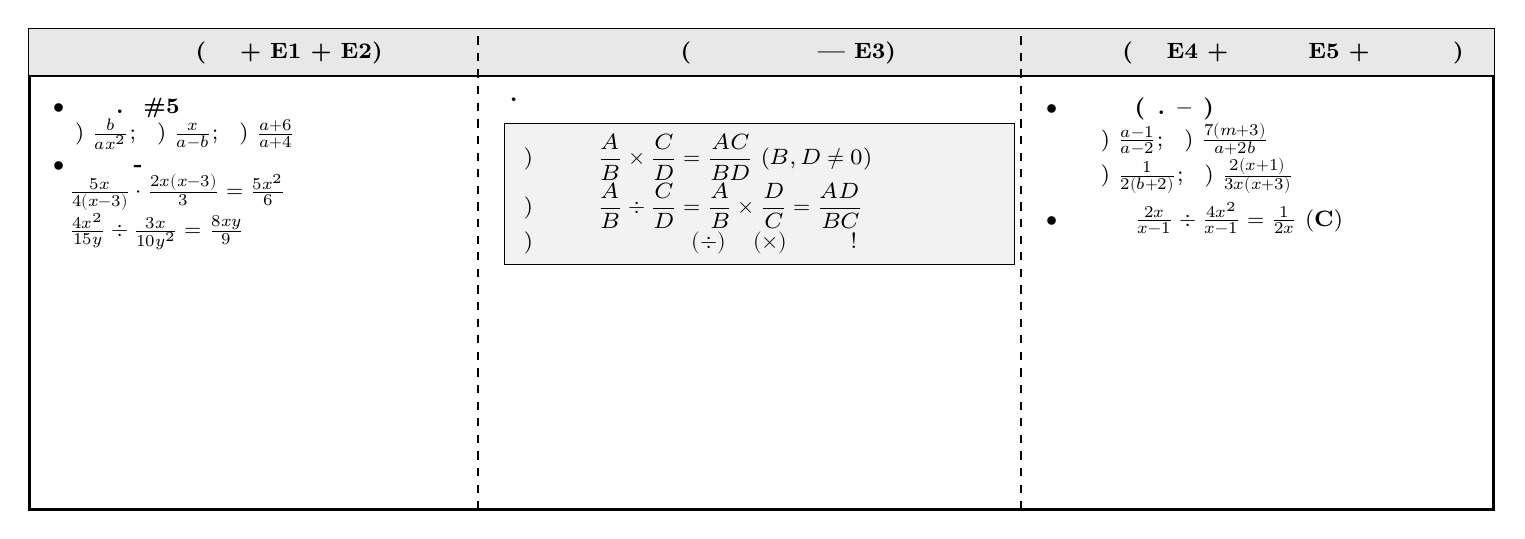
\begin{tikzpicture}[x=1cm, y=1cm, every node/.style={font=\footnotesize, text=black}]
  \draw[black, line width=1.1pt] (0,0) rectangle (18.6,6.1);
  \fill[gray!18] (0,5.50) rectangle (18.6,6.1);
  \draw[black, line width=0.7pt] (0,5.50) -- (18.6,5.50);
  \draw[black, dashed, line width=0.75pt] (5.7,0) -- (5.7,6.1);
  \draw[black, dashed, line width=0.75pt] (12.6,0) -- (12.6,6.1);

  \node at (2.85,5.80) {\textbf{ផ្នែកឆ្វេង (កំណែ + \en{E1} + \en{E2})}};
  \node at (9.15,5.80) {\textbf{ផ្នែកកណ្ដាល (ខ្លឹមសារគោលរក្សាទុក — \en{E3})}};
  \node at (15.60,5.80) {\textbf{ផ្នែកស្ដាំ (គំរូ \en{E4} + ប្រតិបត្តិ \en{E5} + កិច្ចការផ្ទះ)}};

  % Left zone
  \node[anchor=north west, text width=5.3cm] at (0.18,5.35) {
    $\bullet$ \textbf{កំណែ ទំ.៨៥ \en{\#5}៖}\\
    \hspace*{0.2cm}ខ) $\tfrac{b}{ax^2}$; \ គ) $\tfrac{x}{a-b}$; \ ឍ) $\tfrac{a+6}{a+4}$\\[2pt]
    $\bullet$ \textbf{ឧទាហរណ៍គុណ-ចែក៖}\\
    \hspace*{0.2cm}$\tfrac{5x}{4(x-3)}\cdot\tfrac{2x(x-3)}{3} = \tfrac{5x^2}{6}$\\
    \hspace*{0.2cm}$\tfrac{4x^2}{15y}\div\tfrac{3x}{10y^2} = \tfrac{8xy}{9}$
  };

  % Center zone
  \node[anchor=north west, text width=6.5cm] at (5.90,5.35) {
    {\muol\fontsize{8.2pt}{12pt}\selectfont ៤\enbf{.} វិធីគុណនិងវិធីចែកកន្សោមសនិទាន}\\[3pt]
    \begin{tcolorbox}[enhanced, sharp corners, colback=gray!10, colframe=black, boxrule=0.6pt, boxsep=1.5pt, left=3pt, right=3pt, top=2pt, bottom=2pt]
      ១) \textbf{វិធីគុណ៖} $\dfrac{A}{B} \times \dfrac{C}{D} = \dfrac{AC}{BD}$ ($B, D \neq 0$)\\
      ២) \textbf{វិធីចែក៖} $\dfrac{A}{B} \div \dfrac{C}{D} = \dfrac{A}{B} \times \dfrac{D}{C} = \dfrac{AD}{BC}$\\
      ៣) ដាក់ជាកត្តាសិន ហើយប្ដូរ $(\div)$ ជា $(\times)$ មុនសម្រួល!
    \end{tcolorbox}
  };

  % Right zone
  \node[anchor=north west, text width=5.6cm] at (12.80,5.35) {
    $\bullet$ \textbf{លំហាត់គំរូ (ទំ.៧៩--៨០)៖}\\
    \hspace*{0.2cm}គុណ៖ ក) $\tfrac{a-1}{a-2}$; \ ខ) $\tfrac{7(m+3)}{a+2b}$\\
    \hspace*{0.2cm}ចែក៖ ក) $\tfrac{1}{2(b+2)}$; \ ខ) $\tfrac{2(x+1)}{3x(x+3)}$\\[2pt]
    $\bullet$ \textbf{វិនិច្ឆ័យ៖} $\tfrac{2x}{x-1}\div\tfrac{4x^2}{x-1} = \tfrac{1}{2x}$ (\textbf{\en{C}})
  };
\end{tikzpicture}
\end{center}

\secstrip{២. ចម្លើយផ្ទៀងផ្ទាត់រហ័សសម្រាប់សន្លឹកកិច្ចការសិស្ស \enbf{(}ទំព័រ ១ និង ទំព័រ ២\enbf{)}}{\en{Answer Key}}

\begin{tcolorbox}[
  enhanced, sharp corners, colback=white, colframe=black,
  boxrule=0.8pt, boxsep=2.5pt, top=4pt, bottom=4pt, left=6pt, right=6pt
]
  $\bullet$ \textbf{ផ្នែក \en{E1}៖} សិស្ស ខ ត្រឹមត្រូវ (តេស្ត $a=6$៖ សិស្ស ក បាន $\tfrac{1}{18} \neq \tfrac{1}{2}$; សិស្ស ខ បាន $\tfrac{9}{18} = \tfrac{1}{2}$ ត្រឹមត្រូវ) ។\\[2pt]
  $\bullet$ \textbf{ផ្នែក \en{E2}៖} សកម្មភាព ១៖ $\tfrac{7a}{16}$; $\tfrac{5x^2}{6}$ ។ សកម្មភាព ២៖ $\tfrac{8xy}{9}$; $\tfrac{(a-3)^2}{3a}$ ។\\[2pt]
  $\bullet$ \textbf{ផ្នែក \en{E4}៖} ១) $\tfrac{a-1}{a-2}$; $\tfrac{7(m+3)}{a+2b}$ ។ ២) $\tfrac{1}{2(b+2)}$; $\tfrac{2(x+1)}{3x(x+3)}$ (ងាយសម្រួលកត្តារួមភ្លាមៗ) ។\\[2pt]
  $\bullet$ \textbf{ផ្នែក \en{E5}៖} ១) $3$; $\tfrac{4}{x+3}$; $1$; $-\tfrac{4p}{2p+q}$; ២) សិស្ស ខ ($\tfrac{1}{2}$); ៣) \textbf{ជម្រើស \en{C}} ($\tfrac{1}{2x}$); ៤) $1$ ។
\end{tcolorbox}

\secstrip{៣. ចម្លើយលម្អិតនៃកិច្ចការផ្ទះ \enbf{(}សម្រាប់គ្រូផ្ទៀងផ្ទាត់នៅដើមម៉ោងបន្ទាប់\enbf{)}}{សៀវភៅគោល ទំ.៨៦}

\begin{tcolorbox}[
  enhanced, sharp corners, colback=white, colframe=black,
  boxrule=0.8pt, boxsep=2.5pt, top=4pt, bottom=4pt, left=6pt, right=6pt
]
  $\bullet$ \textbf{១) ទំ.៨៦ \en{\#6} ក, ខ៖} ក) $\dfrac{-24x^5y^3}{30x^5y^4} = \mathbf{-\dfrac{4}{5y}}$; \quad ខ) $\dfrac{4x}{3y} \times \dfrac{15x^2y^3}{4xy} = \mathbf{5x^2y}$ ។\\[2pt]
  $\bullet$ \textbf{២) ទំ.៨៦ \en{\#6} ង, ឈ, ដ៖} ង) $\mathbf{b(b + 3)}$; \quad ឈ) $(a-7)\cdot\dfrac{(7-a)(7+a)}{(7-a)^2} = \mathbf{-(a + 7)}$; \quad ដ) $\mathbf{\dfrac{b - 4}{b - 3}}$ ។
\end{tcolorbox}

\end{document}
